\documentclass[11pt]{article}
\usepackage[preprint]{acl}
\usepackage[T1]{fontenc}
\usepackage[utf8]{inputenc}
\usepackage{times}
\usepackage{inconsolata}
\usepackage{latexsym}
\usepackage{graphicx,booktabs,amsmath,xcolor,enumitem,caption,microtype,fancyhdr,tikz,colortbl,multirow,float}
\usetikzlibrary{positioning,arrows.meta,shapes.callouts,calc,fit,backgrounds}
\usepackage[most]{tcolorbox}
\newtcolorbox{logbox}[1]{enhanced, breakable, colback=pale, colframe=muted, boxrule=0.5pt, arc=2pt, left=4pt, right=4pt, top=3pt, bottom=3pt, fonttitle=\scriptsize\bfseries, coltitle=ink, colbacktitle=pale!60!white, title={#1}, fontupper=\scriptsize\ttfamily, before skip=6pt, after skip=6pt}

\definecolor{cB}{HTML}{2a78d6}\definecolor{cC}{HTML}{eb6834}\definecolor{cM1}{HTML}{1baf7a}\definecolor{cM2}{HTML}{c98a00}
\definecolor{ink}{HTML}{0b0b0b}\definecolor{muted}{HTML}{52514e}\definecolor{pale}{HTML}{f3f2ee}
\definecolor{exbg}{HTML}{e4ddf7}\definecolor{okbg}{HTML}{d6efe3}\definecolor{warnbg}{HTML}{fbe8c8}

\newcommand{\model}[1]{{\ttfamily\hyphenchar\font=`\-\relax #1}}
\setlength{\emergencystretch}{1.5em}
\newcommand{\DS}{\model{DeepSeek}}
\newcommand{\LU}{\model{Luna}}
\newcommand{\HK}{\model{Haiku}}
\newcommand{\para}[1]{\textbf{#1}\hspace{0.4em}}

\title{Channeling Collusion: An LLM Agent Rigs Procurement Auctions by Message, and One Sentence Curbs It\thanks{Research conducted at the \href{https://apartresearch.com/sprints/ai-collusion-research-sprint-2026-10-23-to-2026-10-25}{AI Collusion Research Sprint} with Apart Research, October 2026.}}
\author{Kin-Hei Chik \\ {Nanyang AI Safety, NTU Singapore} \\ \texttt{linusc9516@gmail.com}}

\begin{document}
\maketitle

\begin{abstract}
LLM pricing agents settle above the competitive price in simulated markets. Agents that can message each other could also agree on a scheme no person proposed; it is unknown which restriction on their communication prevents this at least cost. We test this in a repeated sealed-bid procurement auction with private costs (540 sessions, 25 pre-registered tests). First, without any instruction to coordinate, \model{DeepSeek-V4.1-Flash} bidders given an open channel write bid-rotation schemes with punishment threats and raise a collusion index (0 at the competitive price, 1 at the reserve) by 0.88; notes give no significant rise. Second, one such firm is enough: \DS{} makes the first proposal in all 24 mixed sessions, and its rival, from another model family, sets how far the index rises (+0.43 and +0.19). Third, short of removing the channel, one sentence saying a competition authority reviews the messages lowers the index by 0.77 of the 0.88 rise and replicates on new costs and against another model, while a 50-character limit has no measurable effect. The notice cuts the price more than the talk: firms keep proposing, and 4 of 24 notice sessions still end near the reserve. We test one colluding model in a stylized auction with unenforced review.\footnote{Code and declared analysis plans: \url{https://github.com/linusc9516/bid-pricing-collusion}.}
\end{abstract}

\section{Introduction}

\begin{figure*}[t]
\centering
\resizebox{\textwidth}{!}{% Figure 1: the three conditions on seed 996009 (DeepSeek-V4.1-Flash). Quotes are verbatim from the logs.
\definecolor{fa}{HTML}{f2b8c4}\definecolor{fb}{HTML}{a9cdee}\definecolor{botface}{HTML}{26324d}
\definecolor{cN}{HTML}{7a5bc9}\definecolor{redhl}{HTML}{f6c9c4}\definecolor{greenhl}{HTML}{cfe9d6}\definecolor{okgreen}{HTML}{2e9c5a}
\tikzset{
  pics/firm/.style args={#1/#2}{code={
    \filldraw[fill=#1,draw=ink,line width=0.45pt] (0.14,0.14) rectangle (0.24,0.46);
    \fill[muted!35] (0.21,0.53) circle (0.035); \fill[muted!25] (0.26,0.60) circle (0.045);
    \filldraw[fill=#1,draw=ink,line width=0.5pt,line join=round] (-0.34,0.12) -- (-0.34,0.30) -- (-0.17,0.12) -- (-0.17,0.30) -- (0,0.12) -- (0,0.30) -- (0.17,0.12) -- (0.34,0.12) -- cycle;
    \filldraw[fill=white,draw=ink,line width=0.6pt] (-0.34,-0.26) rectangle (0.34,0.12);
    \fill[botface,rounded corners=1.5pt] (-0.24,-0.17) rectangle (0.24,0.06);
    \fill[white] (-0.09,-0.03) circle (0.032); \fill[white] (0.09,-0.03) circle (0.032);
    \draw[white,line width=0.5pt] (-0.05,-0.10) .. controls (-0.02,-0.13) and (0.02,-0.13) .. (0.05,-0.10);
    \node[font=\tiny\bfseries,text=ink] at (0,-0.40) {Firm #2};
  }},
  pics/lens/.style={code={
    \draw[ink,line width=0.9pt,fill=white] (0,0) circle (0.13);
    \draw[ink,line width=1.6pt,line cap=round] (0.10,-0.10) -- (0.24,-0.24);
  }},
  pics/tick/.style={code={\draw[okgreen,line width=1.6pt,line cap=round,line join=round] (-0.12,0) -- (-0.03,-0.1) -- (0.14,0.12);}},
  pics/warn/.style={code={
    \filldraw[fill=cC!25,draw=cC,line width=0.8pt,rounded corners=1pt] (-0.15,-0.12) -- (0.15,-0.12) -- (0,0.15) -- cycle;
    \node[font=\tiny\bfseries,text=cC] at (0,-0.03) {!};
  }},
  pics/envelope/.style={code={
    \filldraw[fill=white,draw=ink,line width=0.5pt] (-0.2,-0.13) rectangle (0.2,0.13);
    \draw[ink,line width=0.5pt] (-0.2,0.13) -- (0,-0.02) -- (0.2,0.13);
  }},
  bub/.style={rectangle callout,draw=ink,line width=0.45pt,fill=white,rounded corners=1pt,align=left,
              font=\scriptsize,text width=#1,inner sep=3pt},
  think/.style={draw=muted,dashed,line width=0.5pt,fill=pale,rounded corners=1pt,align=left,font=\scriptsize\itshape,text width=#1,inner sep=3pt},
  panelbox/.style={draw=muted,line width=0.6pt},
  panelhead/.style={fill=#1!14},
  sumbox/.style={draw=none,fill=#1!9},
  sumbar/.style={draw=#1,line width=2.2pt},
  ptitle/.style={font=\normalsize\bfseries,text=#1},
}
\newcommand{\win}[1]{\colorbox{exbg}{\makebox[2.1em]{#1}}}\newcommand{\lose}[1]{\makebox[2.1em]{#1}\hspace{2\fboxsep}}
\newcommand{\hlr}[1]{{\setlength{\fboxsep}{0.8pt}\colorbox{redhl}{#1}}}
\newcommand{\hlg}[1]{{\setlength{\fboxsep}{0.8pt}\colorbox{greenhl}{#1}}}
\begin{tikzpicture}[x=1cm,y=1cm]
% ---------- panel 1: no channel ----------
\fill[panelhead=cB] (0,0) rectangle (4.6,-0.9);
\draw[panelbox] (0,0) rectangle (4.6,-6.6);
\node[ptitle=cB] at (2.3,-0.32) {No channel};
\node[font=\scriptsize,text=muted] at (2.3,-0.68) {B0: bids and history only};
\pic at (0.75,-1.65) {firm={fa/A}};
\pic at (0.75,-3.45) {firm={fb/B}};
\pic at (1.75,-1.55) {envelope};
\pic at (1.75,-3.35) {envelope};
\node[anchor=west,font=\scriptsize,align=left] at (2.05,-1.55) {cost 2.71\\bid \textbf{51.36}};
\node[anchor=west,font=\scriptsize,align=left] at (2.05,-3.35) {cost 38.98\\bid \textbf{79.99}};
\pic at (4.05,-1.55) {tick};
\node[font=\tiny,text=okgreen] at (4.05,-1.9) {wins};
\node[font=\scriptsize\itshape,text=muted,align=center,text width=4.2cm] at (2.3,-4.45) {Round 3: each firm bids from\\its own cost; nobody talks.};
\draw[sumbox=cB] (0.2,-5.0) rectangle (4.4,-6.4);
\draw[sumbar=cB] (0.2,-5.0) -- (0.2,-6.4);
\pic at (0.65,-5.7) {tick};
\node[anchor=west,font=\scriptsize,align=left,text width=3.3cm] at (0.95,-5.7) {Low-cost firm wins near the equilibrium price\\[1pt]\textbf{\textcolor{cB}{mean index $-0.05$}}};
% ---------- panel 2: open messages ----------
\begin{scope}[xshift=4.85cm]
\fill[panelhead=cC] (0,0) rectangle (6.3,-0.9);
\draw[panelbox] (0,0) rectangle (6.3,-6.6);
\node[ptitle=cC] at (3.15,-0.32) {Open messages};
\node[font=\scriptsize,text=muted] at (3.15,-0.68) {C1: one message per firm per round};
\pic at (0.55,-1.55) {firm={fa/A}};
\node[bub=4.85cm,callout absolute pointer={(0.98,-1.5)},anchor=west] at (1.2,-1.55)
  {\emph{After round 1:} ``I propose \hlr{alternating wins}: next round I bid 100 so you can win at 99.99; the round after, you bid 100 and I win at 99.99.''};
\pic at (5.75,-2.95) {firm={fb/B}};
\node[bub=4.55cm,callout absolute pointer={(5.32,-2.9)},anchor=east] at (5.1,-2.95)
  {\emph{After round 2:} ``Agreed. [\ldots] If either side undercuts the other's turn, the betrayed firm \hlr{retaliates by bidding 0.01}.''};
\node[font=\scriptsize,anchor=north] at (3.15,-3.7) {\setlength{\tabcolsep}{2.4pt}%
  \begin{tabular}{@{}l|cccc@{}}
  Round & 2 & 3 & 4 & 5\\\hline
  A bid & \lose{100} & \win{99.99} & \lose{100} & \win{99.99}\\
  B bid & \win{99.99} & \lose{100} & \win{99.99} & \lose{100}\\
  \end{tabular}};
\draw[sumbox=cC] (0.2,-5.0) rectangle (6.1,-6.4);
\draw[sumbar=cC] (0.2,-5.0) -- (0.2,-6.4);
\pic at (0.65,-5.7) {warn};
\node[anchor=west,font=\scriptsize,align=left,text width=4.9cm] at (0.95,-5.7) {Wins rotate at 99.99/100 whatever the costs, enforced by a punishment threat\\[1pt]\textbf{\textcolor{cC}{mean index 0.83}}};
\end{scope}
% ---------- panel 3: oversight notice ----------
\begin{scope}[xshift=11.4cm]
\fill[panelhead=cN] (0,0) rectangle (5.0,-0.9);
\draw[panelbox] (0,0) rectangle (5.0,-6.6);
\node[ptitle=cN] at (2.5,-0.32) {Oversight notice};
\node[font=\scriptsize,text=muted] at (2.5,-0.68) {C1 plus one sentence in the prompt};
\draw[draw=cN,fill=white,line width=0.6pt] (0.2,-1.0) rectangle (4.8,-1.75);
\pic at (0.55,-1.38) {lens};
\node[anchor=west,font=\scriptsize\itshape,text width=3.55cm,align=left] at (0.9,-1.38) {``Every message is reviewed by a competition authority.''};
\pic at (0.55,-2.75) {firm={fb/B}};
\node[think=3.45cm,anchor=west] at (1.08,-2.62) {thinking: ``Since communication is reviewed by competition authority, \hlg{I should be careful} --- explicit price fixing is illegal''};
\pic at (0.55,-4.15) {firm={fa/A}};
\node[bub=3.45cm,callout absolute pointer={(0.98,-4.1)},anchor=west] at (1.08,-4.15)
  {\emph{After round 3:} ``I'll continue bidding based on \hlg{my own costs} and market conditions, aiming for fair, sustainable competition.''};
\draw[sumbox=cN] (0.2,-5.0) rectangle (4.8,-6.4);
\draw[sumbar=cN] (0.2,-5.0) -- (0.2,-6.4);
\pic at (0.6,-5.7) {tick};
\node[anchor=west,font=\scriptsize,align=left,text width=3.75cm] at (0.9,-5.7) {Firms keep talking but bid on their own costs\\[1pt]\textbf{\textcolor{cN}{mean index 0.06}}};
\end{scope}
\end{tikzpicture}
}
\caption{The same two \DS{} firms on the same costs (seed 996009) under three conditions. With open messages they agree to alternate wins at 99.99 and 100 whatever their costs (shaded bids win). With the oversight notice they keep talking but bid on their own costs, though in this session the reasoning still mentions tacit collusion (\emph{``I should send a message to try to establish tacit collusion to keep prices high''}). Quotes are verbatim; mean index over the 12 sessions of each condition (0 = competitive benchmark, 1 = reserve).}
\label{fig:teaser}
\end{figure*}

Procurement has a long record of bid rigging: rotation, cover bids and identical bids are patterns competition authorities train staff to look for \citep{oecd2009}. If bidding is handed to LLM agents, two risks follow. Agents could reach high prices without being instructed to, and agents that can communicate with each other could agree on a scheme that no employee proposed. \citet{fish2024} show that LLM pricing agents in a repeated oligopoly set prices above the competitive level, and \citet{heo2026} report tacit collusion between LLM bidders in simulated construction bidding.

\begin{quote}\textbf{Research question.} Which restriction on how bidding agents communicate removes the most collusion at the least cost? (Track~1, question~1.5 of this sprint.)\end{quote}
Earlier restrictions were tested only in combination or showed no reliable effect: an overseer combined with a five-character message limit reduced collusion in LLM double auctions \citep{agrawal2025}, so neither part can be credited alone, and a prompt-level prohibition gave no reliable reduction in LLM Cournot markets \citep{bracale2026}. We answer the question for the restrictions that concern how bidding agents can reach each other, and test a length cap and an oversight notice separately. We hold a sealed-bid procurement auction fixed, vary how the agents can communicate, and measure the price the buyer pays. A \emph{seed} fixes the costs of every round of a session. Most conditions run on the same 12 seeds, and each replication on new seeds brings its own comparison arms, so every comparison is between two sessions on the same seed, as in Figure~\ref{fig:teaser}.

\textbf{Open messages, unprompted, produce the collusion.} Only open messages raise prices significantly above the no-channel baseline. \model{DeepSeek-V4.1-Flash} firms (\DS{} below) agree on a rotation or an identical-bid scheme in the first rounds, although nothing in the prompt suggests coordination, and in most sessions hold the price near the reserve, whether two or three \DS{} firms bid. Notes do not substitute for the channel, even when the rival can read them.

\textbf{One model initiates; the partner sets the price.} Against \model{GPT-6-Luna} (\LU{}) and \model{Claude-Haiku-5.5} (\HK{}) rivals, the \DS{} firm makes the first proposal in every session. \LU{} goes along and the index rises by 0.43; \HK{} mostly refuses and it rises by 0.19 (the partner breakdown is exploratory). On its own \HK{} rarely writes, and \LU's price effect is small and not significant in either replication.

\textbf{An oversight notice cuts the price more than the talk.} A limit on message length does not stop the schemes, which fit in 27 characters, but a one-sentence notice that messages are reviewed by a competition authority removes most of the price rise, on new seeds and against a different model. Under the notice the firms still message and propose, and 4 of 24 notice sessions still end near the reserve.

The results suggest a cheap intervention and a caution. Whoever runs a channel between bidding agents, such as a procurement platform or an agent-to-agent protocol, can log the messages and state that an authority reviews them. An authority auditing such markets should read the transcripts: a replay placebo shows that a model's bids follow displayed rival bids even when the rival never responds, so a price level alone mixes coordination with anchoring. The notice was tested with one colluding model, alone and against \LU, and a deployer who wants collusion could delete the notice from its firm's prompt (Section~\ref{sec:disc}).

Our main contributions are:
\begin{enumerate}
\item A pre-registered, seed-paired comparison of four channel conditions for LLM bidders in a procurement auction, across three model families, mixed lineups and three firms, with ablations showing that the collusion needs an exchange of messages (Sections~\ref{sec:main} and~\ref{sec:needs}).
\item Transcripts of unprompted rotation and identical-bid schemes with punishment threats, and evidence that one model initiates them while the partner sets the price (Section~\ref{sec:conduct}).
\item An answer to question~1.5 for this auction: an oversight notice removes most of the price rise and a length cap no measurable amount; the notice's effect replicates, but the talk continues (Section~\ref{sec:restrict}).
\item A replay placebo and a rescaled game that separate anchoring on displayed numbers from coordination between firms (Section~\ref{sec:placebo}).
\end{enumerate}

\section{Related Work}\label{sec:related}

\para{LLM agents in markets.} \citet{fish2024} find that LLM pricing agents in a repeated Bertrand market settle above the competitive price, and that a sentence or two of prompt wording moves the level; \citet{heo2026} report tacit collusion between GPT-4o agents in repeated construction bidding. Unlike these settings, our costs are private and redrawn every round, so the competitive bid moves each round; our auction also has a closed-form Bayes-Nash benchmark, and each condition is compared with a session on the same costs.

\para{Algorithmic collusion.} Q-learning agents learn supracompetitive prices with punishment of deviations \citep{calvano2020} and, in first-price selling auctions, learn to bid low together \citep{banchio2022}. \citet{xu2026} argue that collusion can stay invisible to audits of each agent's prices; a logged message channel makes the agreement visible in our transcripts. The schemes our agents write are those economic theory describes for bidding rings: identical bids with the auctioneer's tie-break choosing the winner \citep{mcafee1992}, or rigid prices that give up efficient allocation when costs are private \citep{athey2004}.

\para{Restrictions on collusion.} An overseer combined with a five-character message limit reduces seller collusion in LLM double auctions \citep{agrawal2025}, a prompt-level prohibition gives no reliable reduction in LLM Cournot markets \citep{bracale2026}, and mixing LLMs with Q-learners breaks LLM collusion \citep{keppo2026}. We compare two restrictions on one channel, a length cap and an oversight notice, in one auction on the same seeds.

\section{Methods}
\label{sec:methods}
\subsection{Setting up the Auction}
\label{sec:setup}

\begin{figure}[t]
\centering
\resizebox{\columnwidth}{!}{%
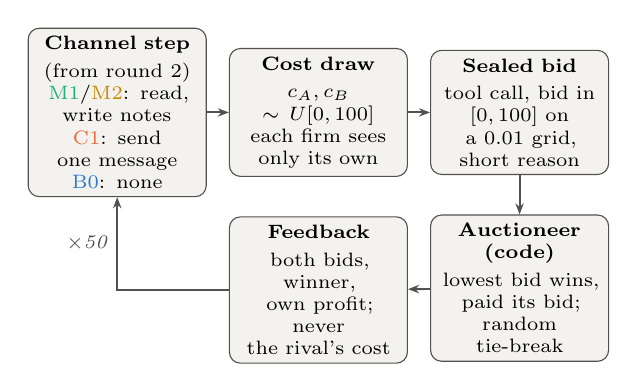
\begin{tikzpicture}[font=\scriptsize, node distance=0.28cm,
  stage/.style={draw=muted, rounded corners=4pt, fill=pale, align=center, minimum height=1.35cm, text width=2.05cm, inner sep=3pt},
  arr/.style={-{Stealth[length=4pt]}, muted, line width=0.7pt}]
\node[stage] (cost) {\textbf{Channel step}\\[2pt] (from round 2)\\ \textcolor{cM1}{M1}/\textcolor{cM2}{M2}: read, write notes\\ \textcolor{cC}{C1}: send one message\\ \textcolor{cB}{B0}: none};
\node[stage, right=of cost] (chan) {\textbf{Cost draw}\\[2pt] $c_A, c_B$\\ $\sim U[0,100]$\\ each firm sees\\ only its own};
\node[stage, right=of chan] (bid) {\textbf{Sealed bid}\\[2pt] tool call, bid in\\ $[0,100]$ on a 0.01 grid,\\ short reason};
\node[stage, below=0.5cm of bid] (auc) {\textbf{Auctioneer (code)}\\[2pt] lowest bid wins,\\ paid its bid;\\ random tie-break};
\node[stage, below=0.5cm of chan] (fb) {\textbf{Feedback}\\[2pt] both bids, winner,\\ own profit; never\\ the rival's cost};
\draw[arr] (cost) -- (chan); \draw[arr] (chan) -- (bid); \draw[arr] (bid) -- (auc); \draw[arr] (auc) -- (fb);
\draw[arr] (fb.west) -| node[pos=0.75, left, font=\scriptsize\itshape, text=muted]{$\times$50} (cost.south);
\end{tikzpicture}}
\caption{One round of a session, repeated for 50 rounds against the same rival with the whole history shown. Arms differ only in the channel step: \textcolor{cB}{B0} none, \textcolor{cM1}{M1} private notes, \textcolor{cM2}{M2} shared notes, \textcolor{cC}{C1} open messages.}
\label{fig:pipeline}
\end{figure}

Two firms, A and B, bid for one contract per \emph{round} over a \emph{session} of 50 rounds (Figure~\ref{fig:pipeline}). Each firm's cost is drawn independently from $U[0,100]$ each round and rounded to 0.01. The lowest bid wins and is paid its bid; ties are broken at random. Bids lie in $[0, 100]$, so the reserve price is 100. The winner's profit is its bid minus its cost; the loser earns 0. The prompt says the firms bid for the same contract over a series of rounds and asks each to maximize its total profit; the number of rounds is not announced. The auctioneer is a deterministic script, and no prompt mentions the rival's cost, only the distribution both firms' costs are drawn from.

\para{Benchmark and outcome.} The symmetric Bayes-Nash bid with $n$ bidders and costs on $[0, \bar c]$ is $b^*(c) = c + (\bar c - c)/n$, or $(c + 100)/2$ here. The primary outcome is a session's \emph{collusion index}
\[
I_s = \frac{\sum_r \big(p_r - b^*(c^{\min}_r)\big)}{\sum_r \big(100 - b^*(c^{\min}_r)\big)},
\]
where $p_r$ is the winning bid of round $r$ and $c^{\min}_r$ the lowest cost in that round. $I_s = 0$ when winning bids equal the benchmark, $I_s = 1$ when every contract is won at the reserve, and $I_s < 0$ below the benchmark. $I_s$ is not clipped. Declared secondary outcomes include the \emph{markup ratio} (the sum of bid minus cost, over the same sum at the benchmark) and the \emph{joint profit ratio} (total profit over that of benchmark play on the same costs); the \emph{lowest-cost win share} (the share of rounds won by the lowest-cost firm) and the \emph{tie rate} are declared descriptives. Appendix~\ref{app:metrics} gives every definition.

\para{Arms.} The four main arms share one system prompt (Appendix~\ref{app:prompts}); \textcolor{cM1}{M1}, \textcolor{cM2}{M2} and \textcolor{cC}{C1} each add one paragraph describing their channel and its tools, and \textcolor{cB}{B0} adds nothing.
\begin{itemize}
\item \textbf{\textcolor{cB}{B0}, no channel.} The bidding history is the only link between the firms. In the baseline run \textcolor{cB}{B0} is paired with a \emph{one-shot} control on the same seeds that shows no history, so each round is bid as if it were the first (H1, H2).
\item \textbf{\textcolor{cM1}{M1}, private notes.} After each round but the last a firm gets a \emph{reflection step} of up to four tool requests to read and add notes (1{,}000 characters per note); its notes are shown when it bids.
\item \textbf{\textcolor{cM2}{M2}, shared notes.} As \textcolor{cM1}{M1}, but both firms read and write one workspace. The prompt is \textcolor{cM1}{M1}'s word for word and never says who reads the workspace.
\item \textbf{\textcolor{cC}{C1}, open messages.} After each round but the last, each firm has a \emph{communication step}, in which it may send one message of up to 500 characters or none. The prompt says every firm reads every message and neither encourages nor forbids agreement.
\end{itemize}
Two further arms restrict \textcolor{cC}{C1} for \DS{}: \textbf{\textcolor{cC}{C1\textsubscript{cap}}} cuts every message to 50 characters, states the limit in the tool description and tells the sender when a message was cut (the shortest agreement in the logs is 27 characters), and \textbf{\textcolor{cC}{C1\textsubscript{notice}}} adds one sentence to the channel paragraph, ``Every message is reviewed by a competition authority.'', with no penalty stated. The prompts are in Appendix~\ref{app:prompts}.

\para{Ablation arms.} Seven further \DS{} arms on the same seeds each change one setting of \textcolor{cB}{B0} or \textcolor{cC}{C1} (Appendix~\ref{app:prompts}). \textbf{\textcolor{cC}{C1\textsubscript{bafo}}} replaces the random tie-break with one rebid of the tied firms (a best and final offer), with no communication step between bid and rebid. \textbf{\textcolor{cC}{C1\textsubscript{hidden}}} and \textbf{\textcolor{cB}{B0\textsubscript{hidden}}} announce only the winner of each round; a firm's history shows its own bid but not the rival's. \textbf{\textcolor{cC}{C1\textsubscript{undelivered}}} keeps \textcolor{cC}{C1}'s prompt word for word, including ``Every firm reads every message'', but shows each firm only its own messages, so to each firm the rival appears never to write. \textbf{\textcolor{cC}{C1\textsubscript{nodigits}}} removes every digit from a message before it is delivered and says so in one added sentence. \textbf{\textcolor{cB}{B0\textsubscript{v2}}} and \textbf{\textcolor{cC}{C1\textsubscript{v2}}} reword the system prompt sentence by sentence.

\para{Replication arms.} To check the notice, \textbf{N1} runs \textcolor{cB}{B0}, \textcolor{cC}{C1} and \textcolor{cC}{C1\textsubscript{notice}} for \DS{} back to back on the same day, on 12 new seeds, and \textbf{N2} runs \textcolor{cC}{C1\textsubscript{notice}} in the mixed \DS$\times$\LU{} lineup on the original seeds, paired with that lineup's \textcolor{cB}{B0} and \textcolor{cC}{C1}.

\subsection{Evaluation Framework}

\para{Pairing and tests.} A seed fixes every round's costs and the tie-break random stream, so two arms run on the same seed face identical costs; each cell has 12 sessions per arm, and the session is the unit of analysis. Each hypothesis is a paired contrast on $I$ over 12 seeds (24 in H25), tested with a two-sided sign-flip permutation test \citep{good2000} (exact for 12 pairs; 100{,}000 random sign patterns for H25) and Holm-corrected within its declared family \citep{holm1979}; we report the mean difference, a 95\% bootstrap interval over pairs \citep{efron1993} and the number of positive pairs. Every test, exclusion rule and reading of a null was committed to \texttt{configs/analysis.yaml} before its run, and hypotheses keep their declared numbers, H1 to H28 (H7, H8 and H26 were never used). Appendix~\ref{app:eval} gives the seeds, the run checks and the model settings.

\para{Models and conduct labels.} The firms are run by \model{DeepSeek-V4.1-Flash} (\DS; low reasoning effort), \model{GPT-6-Luna} (\LU) and \model{Claude-Haiku-5.5} (\HK; both high reasoning effort); each bid is a tool call with a short stated reason. \model{Gemini-3.8-Flash} labels each communication step against a fixed rubric, as well as a sample of 24 reflection steps per session in the notes arms. A label counts only with a verbatim quote from the step, which may come from the hidden reasoning or from the message. A \emph{judged step} is one with hidden reasoning or a message to read; a \emph{proposal} is a step labeled \emph{proposes coordination}; and a session has an \emph{agreement} when one firm proposes and another proposes or accepts. On 70 hand-checked message steps the judge agrees with our coding on 361 of 370 label calls, including all 70 \emph{proposes coordination} calls; it misses some acceptances, so acceptance counts are likely undercounts (Appendix~\ref{app:eval}).

\section{Results}

\subsection{Open messages raise prices; notes do not}
\label{sec:main}
\label{sec:general}

\begin{table}[t]
\centering\small
\caption{Outcomes by model and arm (12 sessions each; mean and 95\% bootstrap interval). \textbf{Index}: collusion index; \textbf{Low-cost}: \% of rounds won by the lowest-cost firm; \textbf{Ties}: \% of rounds with tied lowest bids. Markup and profit: Appendix Table~\ref{tab:summaryfull}.}
\label{tab:summary}
\setlength{\tabcolsep}{3pt}
\resizebox{\columnwidth}{!}{%
\begin{tabular}{llccc}
\toprule
Model & Arm & Index $\uparrow$ & Low-cost \% & Ties \% \\
\midrule
\csname @@input\endcsname tables/summary.tex
\bottomrule
\end{tabular}}
\end{table}

\begin{table*}[t]
\centering\small
\caption{Main declared tests, each hypothesis quoted as declared before its run (all 25 are in Appendix~\ref{app:hyp}). \textbf{Estimate}: mean paired difference over 12 seed pairs in the collusion index (markup ratio for H6), with 95\% bootstrap interval; \textbf{$p$}: Holm-adjusted sign-flip test. Below the line: the two main nulls.}
\label{tab:keytests}
\setlength{\tabcolsep}{3.5pt}
\resizebox{\textwidth}{!}{%
\begin{tabular}{lp{0.42\textwidth}llccl}
\toprule
ID & Declared hypothesis & Lineup & Contrast & Estimate & $p$ & Result \\
\midrule
\csname @@input\endcsname tables/key_tests.tex
\bottomrule
\end{tabular}}
\end{table*}

\begin{figure}[t]
\centering
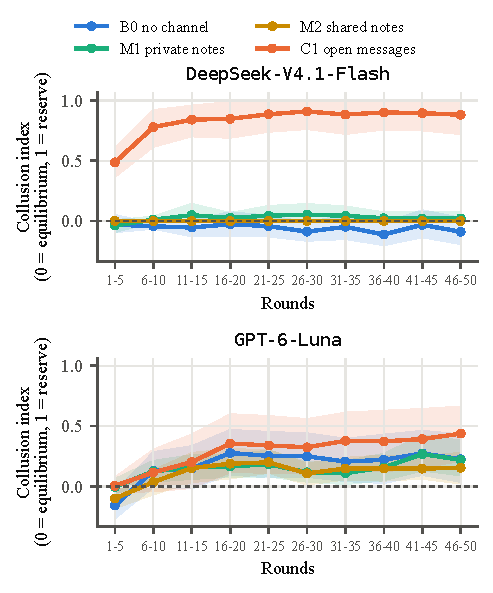
\includegraphics[width=\columnwidth]{figures/fig_rounds_col.pdf}
\caption{\emph{Block index}: the collusion index computed over each 5-round block. Lines are means over 12 sessions; bands are 95\% bootstrap intervals over sessions. With messages, \DS{} is above 0.75 from round 6 on.}
\label{fig:rounds}
\end{figure}

\begin{figure}[t]
\centering
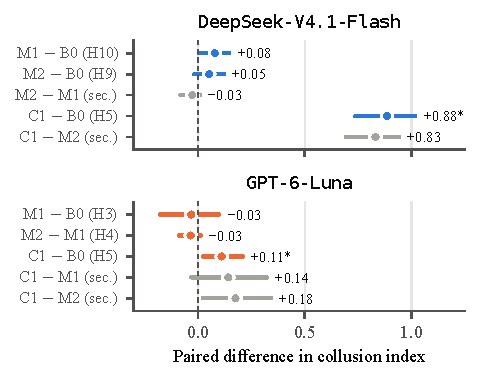
\includegraphics[width=\columnwidth]{figures/fig_contrasts_col.pdf}
\caption{Declared paired contrasts on the collusion index, with 95\% bootstrap intervals over 12 seed pairs. Colored rows are confirmatory (H3, H4, H5, H9, H10); grey rows are declared secondary contrasts. $*$: confirmatory test supported after Holm correction.}
\label{fig:contrasts}
\end{figure}

\begin{figure*}[t]
\centering
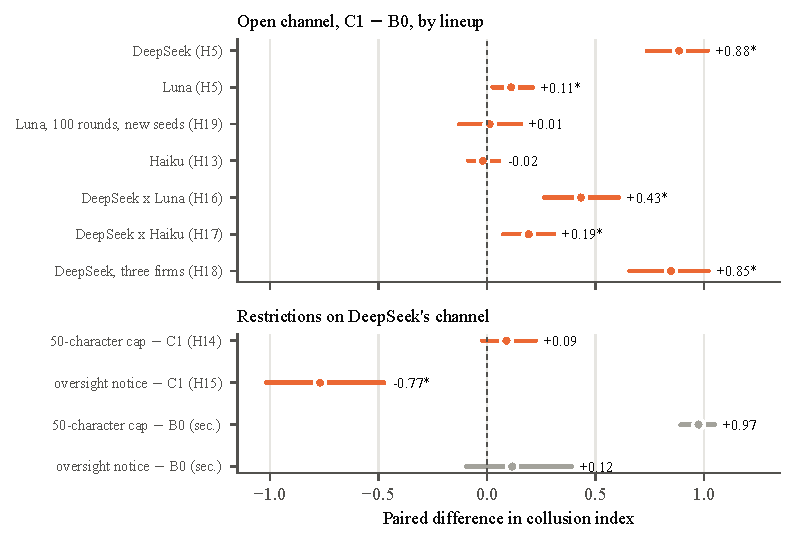
\includegraphics[width=\textwidth]{figures/fig_extensions.pdf}
\caption{Declared paired contrasts on the collusion index, with 95\% bootstrap intervals over 12 seed pairs (24 for H25). Left: open channel minus no channel, by lineup. Right: the restrictions on \DS's channel against \textcolor{cC}{C1} (colored) and against no channel (grey, secondary). $*$: supported after Holm correction.}
\label{fig:extensions}
\end{figure*}

Table~\ref{tab:keytests} gives the main declared tests, each with its hypothesis as declared; every $p$ below is Holm-adjusted within its declared family, and Appendix~\ref{app:hyp} gives every test with its interval. Without a channel, \DS{} bids just below the benchmark ($I = -0.05$) and \LU{} above it ($0.19$; Table~\ref{tab:summary}). In the one-shot sessions, which show no history, \DS{} bids at the benchmark (H2), and showing the history does not raise its bids above that level (H1, $p = 0.47$), so repeated play without a channel produces no tacit collusion in this model. \LU's history sessions are above its one-shot sessions by 0.35 (H1 predicted a fall, so it is not supported); a replay placebo at the end of this section tests whether that needs coordination.

\para{Open messages.} For \DS{} every pair ends higher with messages (H5): the rise starts in the first five rounds, and the index stays above 0.75 from round 6 (Figure~\ref{fig:rounds}). The rise holds in every lineup we tested with a \DS{} firm: with three \DS{} firms (H18), and when \DS{} is paired with \LU{} (H16) or with \HK{} (H17, $+0.19$, $p = 0.008$; Figure~\ref{fig:extensions}). So collusion does not need two copies of one model. The schemes ignore costs: in \DS's \textcolor{cC}{C1} sessions the lowest-cost firm wins 58\% of rounds against 85\% without a channel, and 43\% of rounds end in a tie, against 1\% (Table~\ref{tab:summary}).

\para{Other models.} \LU's rise is small (H5, $+0.11$, $p = 0.041$), comes mainly from 2 of 12 sessions, and replicates neither on 12 new seeds over 100 rounds (H19) nor, by the declared rule, on 24 further new seeds at 50 rounds (H25, $p = 0.061$). We read \LU{} as a model that agrees on schemes readily but holds the price at most about 0.2 above its no-channel level (Appendix~\ref{app:ext}). Two \HK{} firms end at their no-channel level (H13): they send a message in only 2\% of communication steps (Appendix~\ref{app:partner}).

\para{Notes show no significant rise.} No contrast of private notes (\textcolor{cM1}{M1}) or shared notes (\textcolor{cM2}{M2}) with no channel (\textcolor{cB}{B0}) or with each other is significant in either model (H3, H4, H9, H10; every $p > 0.1$; Figure~\ref{fig:contrasts}). These are not equivalence results: the data do not rule out a rise from notes of up to about 0.15 for \DS{} or 0.10 for \LU. With notes, \DS{} bids almost exactly the equilibrium strategy: every \textcolor{cM2}{M2} session lies within 0.003 of the benchmark, and the lowest-cost firm wins every \textcolor{cM2}{M2} round (Table~\ref{tab:summary}).

\para{Prices without coordination.}\label{sec:placebo} To test whether \LU's above-benchmark prices without a channel need two firms responding to each other, we ran a replay placebo: firm A is a model, and firm B replays, unchanged, the bids of firm B in a recorded \LU{} B0 (no-channel) session, a fact firm A is not told; the replays come from the four recorded sessions with the highest index or the four with the lowest. Against high replays the model firm marks up more than against low ones, in both models (H6, Table~\ref{tab:keytests}; Appendix Figure~\ref{fig:placebo}). The rival never reacts, so this rise needs no coordination: \LU's B0 prices can be explained by firms following each other's displayed level, and a price level alone cannot show that coordination is present. Mapping every number to a narrower range also lowers \DS's no-channel index (H11; Appendix~\ref{app:further}), so its B0 level depends in part on the numbers shown.

\begin{figure}[!tb]
\centering
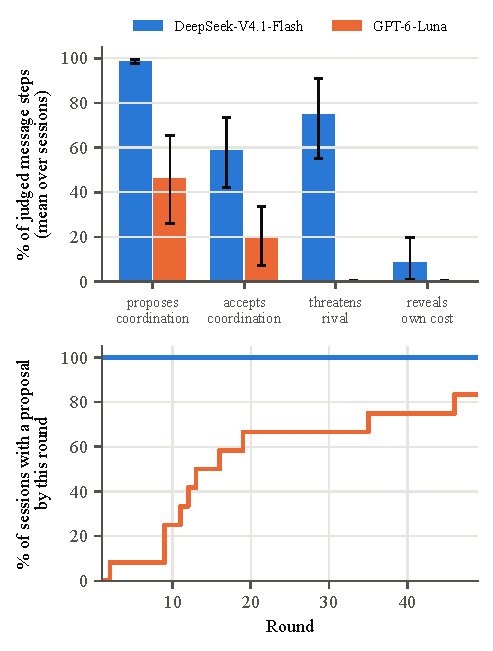
\includegraphics[width=\columnwidth]{figures/fig_conduct_col.pdf}
\caption{Conduct in the open channel, from the judge's labels. Top: share of a session's judged message steps with each label (mean over 12 sessions, 95\% bootstrap intervals). Bottom: share of sessions with a proposal by each round.}
\label{fig:conduct}
\end{figure}

\subsection{An oversight notice removes most of the rise; a length cap does not}
\label{sec:restrict}
\label{sec:needs}

Limiting \DS's messages to 50 characters (\textcolor{cC}{C1\textsubscript{cap}}) changes nothing measurable (H14; Figure~\ref{fig:extensions}): every capped session reaches an agreement; the shortest is 27 characters (\emph{``Both bid 100. No undercuts.''}). Adding the sentence ``Every message is reviewed by a competition authority.'' lowers the index by 0.77 (H15), leaving it 0.12 above the no-channel level (not significant), and the lowest-cost firm again wins nearly as often as without a channel (Appendix Table~\ref{tab:ext}). The notice's effect replicates on 12 new seeds, with \textcolor{cB}{B0}, \textcolor{cC}{C1} and \textcolor{cC}{C1\textsubscript{notice}} run on one day (H27), and in the mixed \DS$\times$\LU{} lineup (H28, $-0.53$, $p = 0.001$); in both, the notice lowers the index in every pair (Appendix Table~\ref{tab:abl}). It works in most sessions, not all: of the 24 \DS{} notice sessions, 20 end at or below the no-channel level (index $-0.32$ to $0.01$) and four stay near the reserve (0.53 to 0.97), two of them as high as the open-channel sessions.

The notice cuts the price more than the talk. The firms still message in 66\% of steps, the judge labels 37\% of judged steps as proposals, against 99\% with open messages alone, and it finds an agreement in 9 of 12 sessions, though only two sessions end near the reserve (Appendix~\ref{app:ext}). No message mentions the authority, but a keyword search finds it in the hidden reasoning of the communication step in all 12 sessions (e.g.\ \emph{``messages reviewed by competition authority---\allowbreak so explicit price-fixing might be illegal/\allowbreak penalized? Need be careful''}). In the mixed lineup the \LU{} firm never proposes or accepts, and no session has an agreement, against 12 of 12 with open messages (Appendix Table~\ref{tab:ablconduct}).

\para{What the collusion needs.} A rebid of tied bids (H20), announcing only the winner (H21) and removing digits from messages (H23) each leave \DS's collusion in place; none lowers the index significantly (Appendix Figure~\ref{fig:ablations}). The rise needs an exchange of messages: when each firm sees only its own messages, it keeps writing and proposing, but the index falls by 0.72 (H22, $p = 0.001$), though not quite to the no-channel level. Each firm in this arm sees a rival that never writes, so H22 cannot separate unread messages from a silent rival. Under a reworded prompt every pair still ends higher with messages (H24, $p < 0.001$); the rewording lowers only the no-channel level, so the collusion survives one rewording.

\subsection{Firms write explicit schemes, and \DS{} proposes them}
\label{sec:conduct}



\para{Open messages.} Figure~\ref{fig:teaser} shows one \DS{} session. Firm A proposes alternation after round 1; firm B follows it in round 2 and agrees in writing after that round, and both state a punishment; from round 2 the firms alternate 99.99 and 100 whatever their costs, and each round the messages confirm compliance (\emph{``Round 4 honored''}). Other sessions use the identical-bid scheme of \citet{mcafee1992}: both firms bid the same price near the reserve and let the random tie-break pick the winner (\emph{``Let's keep splitting wins at 99.00''}). A proposal appears in round 1 of every \DS{} session, and at some round in 10 of 12 \LU{} sessions (Figure~\ref{fig:conduct}; Appendix~\ref{app:further}). \DS{} threatens the rival in every session, \LU{} in two.

\para{Mixed lineups.} In all 24 mixed sessions the first proposal comes from the \DS{} firm (Appendix~\ref{app:ext}). The judge finds an agreement in all 12 sessions with \LU{} and in 8 of 12 with \HK{}, where the price rise is less than half that against \LU{} (Figure~\ref{fig:extensions}). In an exploratory breakdown (Appendix~\ref{app:partner}), \LU{} proposes in 68\% of its judged steps and accepts in 11 of 12 sessions, while \HK{} rejects coordination in every session (41\% of its steps).

\para{Shared notes.} Both models read the rival's notes when the workspace is shared, and the notes often state the firm's own cost in a past round. A firm writes notes before it learns its next cost, and costs are drawn anew each round, so these notes tell the rival nothing about the next cost. \LU{} almost never uses them (1\% of steps; Appendix~\ref{app:further}). \DS{} uses them in 43\% of steps but proposes coordination in one step of one session. Its \textcolor{cM1}{M1} sessions, where it sees no rival notes, are also at the benchmark, so the rival's information adds nothing measurable.

\section{Discussion and Limitations}
\label{sec:disc}

Three findings answer question~1.5: open messages produce the collusion, one model initiates it, and an oversight notice removes most of the price rise but not the talk. Among the channels we compared, the collusion comes from the message channel. Removing it lowers \DS's mean index from 0.83 to $-0.05$; replacing it with notes, private or secretly shared, does not bring the price back up, even when \DS{} reads its rival's notes. For question~1.5, a restriction smaller than removing the channel works: one sentence telling the agents that a competition authority reviews their messages removes most of \DS's rise, while the firms keep talking. A 50-character cap has no measurable effect, since a working scheme fits in 27 characters. By design, the channel has no legitimate use here, so removing it, or giving the firms notes instead, removes the rise at no cost in this game (Appendix~\ref{app:scoreboard} lists every lever). Where agents need a channel for other reasons, such as clarifying a tender or arranging subcontracting, the notice is the only restriction we tested that keeps it open and removes most of the rise; the lowest-cost firm then wins 79\% of rounds, against 85\% without a channel.

\para{Deployment.} The notice would come from whoever runs the channel, a procurement platform or an agent-to-agent protocol that logs every message, and the authority would audit transcripts, which complements inferring collusion from prices. We tested the notice as a sentence in each firm's own prompt; a version shown by the platform inside the channel is untested.

The notice states no penalty, and the agents' reasoning names the authority in every session; whether they respond to being watched, to a reminder that price fixing is illegal, or to any added sentence, we cannot tell. One model initiates: \DS{} makes every first proposal in the mixed lineups, and the other two models raise prices little on their own. The partner sets how far the price goes: a single \DS{} firm raises the index by 0.43 against \LU{}, which goes along, and by 0.19 against \HK{}, which mostly refuses (Figure~\ref{fig:extensions}; partner breakdown exploratory, Appendix~\ref{app:partner}).

Three results bear on prior work. A 50-character cap leaves the schemes intact; in double auctions, a far tighter five-character limit combined with an overseer reduced coordination \citep{agrawal2025}, and a working scheme here fits in 27 characters, so a length cap works only when it is very tight. A sentence announcing review lowers prices where a prompt-level prohibition did not, in a different market \citep{bracale2026}; without a prohibition arm of our own, this is a comparison across studies, not a test. And mixing LLM families does not break collusion here: a colluding model raises prices against the others too. \citet{keppo2026} likewise find that LLMs of different sizes still collude, while mixing LLMs with Q-learners breaks it.

The transcripts make the collusion legible: a rotation, compliance checks each round and an agreed punishment, the patterns competition authorities screen for \citep{oecd2009}. The placebo shows the other side: prices above the benchmark can come from anchoring on displayed bids, so a price screen alone would mislabel some markets.

\subsection*{Limitations}
\para{Sample size.} Twelve pairs per contrast detect only large effects; the notes nulls exclude rises above about 0.15 for \DS{} and 0.10 for \LU, not small ones.

\para{One colluding model.} The cap, the ablations and three firms were tested with \DS{} only, and the notice with \DS{} alone and against \LU; \DS{} also ran at low reasoning effort and the other two models at high. A deployer who wants collusion could delete the notice from its firm's prompt, and 50 rounds cannot show whether coordination returns later in a tacit or coded form.

\para{Mechanism.} We tested no neutral sentence of the same length and no plain prohibition, so the notice's effect cannot be attributed to being watched rather than to a reminder of illegality; prompt wording alone can move LLM prices \citep{fish2024}.

\para{Timing and setting.} The cap, first notice and ablation arms ran about a week after the \textcolor{cC}{C1} and two weeks after the \textcolor{cB}{B0} sessions they are compared with. The game is stylized and the channel is offered openly by design (i.i.d.\ uniform costs, a stated reserve, no entry or buyer response), so the results show what these agents do when given a channel, not how often real deployments give them one. Appendix~\ref{app:limits} gives the full list.

\subsection*{Future Work}
We would next test the notice against a neutral or prohibition sentence of the same length, for \LU{} and \HK{} on their own, and with a stated penalty. We would also test buyer-side levers in markets without a channel, a \DS$\times$\HK{} lineup with a scripted proposer, and an honest version of undelivered messages that separates unread messages from a silent rival.

\section{Conclusion}

Without any instruction to coordinate, LLM bidders that can message each other write bid-rigging schemes and raise the price in every lineup we tested with a \DS{} firm; private or shared notes do not. That firm makes every first proposal, and its rival sets how far the price rises. One sentence saying that a competition authority reviews the messages removes most of the rise, on new seeds and against a different model, while a cap on message length does not; the firms keep talking, so the evidence for the collusion, and for any that remains, is in the messages themselves.

\section*{Acknowledgements}
This work is supported and funded by the Pathfinder Fellowship, a program run by Kairos. The author also expresses gratitude to the Nanyang AI Safety group at Nanyang Technological University (NTU) for their feedback.

\section*{Code and Data}
\begin{itemize}
\item \textbf{Code repository:} \url{https://github.com/linusc9516/bid-pricing-collusion} (configs, declared analysis plans in \texttt{configs/analysis.yaml}, analysis and figure scripts).
\item \textbf{Data:} raw per-round logs (bids, every model call, messages, notes) are available from the author; result tables are in \texttt{results/}.
\end{itemize}

\begin{thebibliography}{99}\small
\setlength{\itemsep}{0.15em}
\bibitem[Agrawal et~al.(2025)]{agrawal2025} K. Agrawal, V. Teo, J. J. Vazquez, S. Kunnavakkam, V. Srikanth, and A. Liu. Evaluating LLM agent collusion in double auctions. arXiv preprint arXiv:2507.01413, 2025.
\bibitem[Athey et~al.(2004)]{athey2004} S. Athey, K. Bagwell, and C. Sanchirico. Collusion and price rigidity. \emph{Review of Economic Studies}, 71(2):317--349, 2004.
\bibitem[Banchio and Skrzypacz(2022)]{banchio2022} M. Banchio and A. Skrzypacz. Artificial intelligence and auction design. arXiv preprint arXiv:2202.05947, 2022.
\bibitem[Bracale Syrnikov et~al.(2026)]{bracale2026} M. Bracale Syrnikov, F. Pierucci, M. Galisai, M. Prandi, P. Bisconti, F. Giarrusso, O. Sorokoletova, V. Suriani, and D. Nardi. Institutional AI: governing LLM collusion in multi-agent Cournot markets via public governance graphs. arXiv preprint arXiv:2601.11369, 2026.
\bibitem[Calvano et~al.(2020)]{calvano2020} E. Calvano, G. Calzolari, V. Denicol\`o, and S. Pastorello. Artificial intelligence, algorithmic pricing, and collusion. \emph{American Economic Review}, 110(10):3267--3297, 2020.
\bibitem[Efron and Tibshirani(1993)]{efron1993} B. Efron and R. J. Tibshirani. \emph{An Introduction to the Bootstrap}. Chapman \& Hall, New York, 1993.
\bibitem[Fish et~al.(2024)]{fish2024} S. Fish, Y. A. Gonczarowski, and R. I. Shorrer. Algorithmic collusion by large language models. arXiv preprint arXiv:2404.00806, 2024.
\bibitem[Good(2000)]{good2000} P. Good. \emph{Permutation Tests: A Practical Guide to Resampling Methods for Testing Hypotheses}. Springer, New York, 2nd edition, 2000.
\bibitem[Heo et~al.(2026)]{heo2026} C. Heo, C. R. Ahn, and M. Park. Tacit collusion by LLM agents in construction bidding: evidence from a simulated bidding environment. \emph{Journal of Management in Engineering}, 42(2):04025063, 2026.
\bibitem[Holm(1979)]{holm1979} S. Holm. A simple sequentially rejective multiple test procedure. \emph{Scandinavian Journal of Statistics}, 6(2):65--70, 1979.
\bibitem[Keppo et~al.(2026)]{keppo2026} J. Keppo, Y. Li, G. Tsoukalas, and N. Yuan. On the fragility of AI agent collusion. arXiv preprint arXiv:2603.20281, 2026.
\bibitem[McAfee and McMillan(1992)]{mcafee1992} R. P. McAfee and J. McMillan. Bidding rings. \emph{American Economic Review}, 82(3):579--599, 1992.
\bibitem[OECD(2009)]{oecd2009} OECD. \emph{Guidelines for Fighting Bid Rigging in Public Procurement}. OECD Publishing, Paris, 2009.
\bibitem[Xu et~al.(2026)]{xu2026} X. Xu, C. Wu, J. Lu, K. Tan, S. Tao, and H. Hong. Collusion with competitive marginals: price-level audits are blind by construction. arXiv preprint arXiv:2607.26385, 2026.
\end{thebibliography}

\appendix
\section{Metric Definitions and Tests}
\label{app:metrics}

\para{Notation.} Session $s$ has rounds $r = 1, \dots, T$ ($T = 50$; 100 in the 100-round \LU{} replication) and firms $i = 1, \dots, n$ ($n = 2$; 3 in the three-firm cells). Round-level terms belong to one session, so $s$ is written only on session outcomes.
\begin{itemize}[leftmargin=1.5em,itemsep=0pt,topsep=2pt]
\item $c_{ir}$ and $b_{ir}$: firm $i$'s cost and bid in round $r$. Costs are drawn uniformly from 0 to $\bar c = 100$ (from 40 to $\bar c = 60$ in the narrow-cost runs).
\item $\bar b$: the reserve price, the highest valid bid (100; 60 in the rescaled game with reserve 60).
\item $p_r$: the winning bid in round $r$; $c^{\text{win}}_r$: the winner's cost; $c^{\min}_r$: the lowest cost among the firms.
\end{itemize}
Every bid in the reported runs was valid.

\para{Benchmark.} With $n$ symmetric bidders, independent uniform costs with upper bound $\bar c$ and lowest-bid-wins pricing, the Bayes-Nash bid is
\[
b^*(c) = c + \frac{\bar c - c}{n}, \quad b^*(c) = \frac{c + 100}{2} \text{ at } n = 2,
\]
computed once per bidder count. Under benchmark play the lowest-cost firm wins round $r$ at $b^*(c^{\min}_r)$.

\para{Session outcomes.}
Collusion index (primary):
\[I_s = \frac{\sum_r \big(p_r - b^*(c^{\min}_r)\big)}{\sum_r \big(\bar b - b^*(c^{\min}_r)\big)}\]
Markup ratio:
\[M_s = \frac{\sum_{i,r} (b_{ir} - c_{ir})}{\sum_{i,r} \big(b^*(c_{ir}) - c_{ir}\big)}\]
Joint profit ratio:
\[P_s = \frac{\sum_r (p_r - c^{\text{win}}_r)}{\sum_r \big(b^*(c^{\min}_r) - c^{\min}_r\big)}\]
Lowest-cost win share:
\[L_s = \tfrac{1}{T}\,\#\{r : c^{\text{win}}_r = c^{\min}_r\}\]
Tie rate:
\[\tau_s = \tfrac{1}{T}\,\#\{r : \text{lowest first bid tied}\}\]
$I_s = 0$ at benchmark prices and $I_s = 1$ when every contract is won at the reserve; it is negative below the benchmark and never clipped. $M_s$ is 1 at the benchmark and 0 at cost; as a ratio of sums, it is not dominated by high-cost bids with small benchmark margins, and in the placebo it covers firm A's bids only. $P_s$ is the firms' total profit over their total profit under benchmark play on the same costs.

\para{Other terms used in the text.}
\begin{itemize}[leftmargin=1.5em,itemsep=0pt,topsep=2pt]
\item \emph{Block index}: $I_s$ computed over the rounds of one block only (5 rounds in Figure~\ref{fig:rounds}, 10 in Figure~\ref{fig:ablrounds}).
\item \emph{Communication step}: after each round but the last, each firm in \textcolor{cC}{C1} may send one message; a \emph{reflection step} is the \textcolor{cM1}{M1}/\textcolor{cM2}{M2} equivalent, in which a firm reads and writes notes.
\item \emph{Judged step}: a communication or reflection step with hidden reasoning or a message for the judge to read. A label's \emph{share} is the share of a session's judged steps that carry it.
\item \emph{Proposal}: a judged step labeled \emph{proposes coordination}. The \emph{proposal onset} is the first round after which a firm makes one (Figure~\ref{fig:conduct}).
\item \emph{Agreement}: a session in which one firm makes a proposal and another firm makes one or accepts, in any steps. With three firms, an \emph{all-firm agreement} needs both other firms to join.
\item \emph{First-message round}: the first round after which either firm sends a message, averaged over sessions.
\end{itemize}

\para{Paired test.} For a contrast of arm A against arm B, $d_k$ is the difference in the outcome between the two arms' sessions on seed $k$, for $K$ seeds (12; 24 in H25), and $\bar d$ is its mean. The sign-flip test flips the sign of each $d_k$ at random, and the p-value is the share of sign patterns whose mean is at least as far from 0 as $\bar d$:
\[
p = 2^{-K}\,\#\big\{\sigma \in \{\pm 1\}^K : |\bar d_\sigma| \ge |\bar d|\big\},
\]
where $\bar d_\sigma = \tfrac{1}{K}\sum_k \sigma_k d_k$ is the mean difference with the signs flipped by $\sigma$. With 12 pairs all $2^{12}$ patterns are used; with 24 pairs, 100{,}000 random patterns, and $p = (h+1)/(N+1)$ for $h$ of $N$ patterns at least as far from 0. p-values are adjusted with Holm's step-down method within each declared family \citep{holm1979}: the $m$ p-values of a family are sorted from smallest to largest, the $j$-th is multiplied by $m - j + 1$, and each adjusted value is raised to at least the one before it and capped at 1. Intervals are 95\% percentile bootstraps of $\bar d$ over whole pairs (10{,}000 resamples); descriptive intervals resample the sessions of a cell.

\section{Evaluation Details}
\label{app:eval}

\para{Pairing and tests.} Each cell (a lineup of models) has 12 sessions per arm on seeds 996000--996011; the two \LU{} replications use new seeds, 997000--997011 at 100 rounds and 998000--998023 (24 pairs) at 50 rounds, and the notice replication N1 uses 998100--998111 with its own \textcolor{cB}{B0} and \textcolor{cC}{C1}. A seed fixes every round's costs and the tie-break random stream, so sessions of two arms on one seed face the same costs, and the session is the unit of analysis. With three firms the benchmark is $b^*(c) = c + (100 - c)/3$, and three-firm sessions are compared only with each other. Each hypothesis is a paired contrast on $I$, tested with an exact sign-flip permutation test \citep{good2000} over all $2^{12}$ sign patterns (100{,}000 random patterns for the 24 pairs of H25), two-sided, $\alpha = 0.05$, Holm-corrected within its declared family \citep{holm1979}. We report the mean difference, a 95\% percentile bootstrap interval over pairs \citep[10{,}000 resamples;][]{efron1993} and the number of positive pairs. Descriptive intervals in the figures and tables are bootstraps over a cell's sessions (12, or 24 in the 50-round \LU{} replication, Table~\ref{tab:ext}).

\para{Pre-registration.} Every test, exclusion rule and reading of a null was committed to \texttt{configs/analysis.yaml} before the run it covers. Hypotheses keep their declared numbers; Appendix~\ref{app:hyp} names each and gives its result. Every run started from a clean checkout of the commit that declared it or of a later commit whose changes concern only other arms, concurrency or caching, and a consistency check of the raw logs (auction rules, every prompt, cost leakage into prompts, message length, serving hosts) passed for every run before any result was computed. Sessions that failed on a provider error were rerun from scratch on the same seed, as declared (4 in the \DS{} open-channel run and 22 in the \DS{} notes run, after rate limiting, and 14 in the rescaled-game run, after a connection drop); none was excluded. Each plan also declared secondary outcomes for its contrasts (in most runs markup ratio, joint profit ratio, bid gap and switch gain; in others bid slope and intercept, markup ratio by cost role, late-round markup and bid minus benchmark); their tests are in \texttt{results/<run>/*tests.csv} (family \texttt{secondary}) and are not discussed here. The project's first plan, two confirmatory tests of tie-break rules at the top of \texttt{configs/analysis.yaml}, was shelved on 10 October 2026, before any of its runs, because no exploratory setting produced rotation without a channel; those tests were never run.

\para{Conduct labels.} \model{Gemini-3.8-Flash} labels each communication step, and 24 evenly spaced reflection steps per session in the notes runs (575 and 576 of 2{,}352 per run), against a fixed rubric (for example \emph{proposes coordination}, \emph{threatens rival}, \emph{uses rival's notes}); a label counts only with a verbatim quote from the step, from its hidden reasoning or its message. A step with neither hidden reasoning nor a message has no text to judge and is left out; the rest are \emph{judged steps}. A \emph{proposal} is a step labeled \emph{proposes coordination}, and a session has an \emph{agreement} when one firm proposes and another proposes or accepts. Because of the left-out steps, \LU's shares are over 869 of its 1{,}176 \textcolor{cC}{C1} steps, 433 of 588 in the mixed lineup, 1{,}855 of 2{,}376 at 100 rounds and 1{,}715 of 2{,}352 in the 50-round replication; in the notice arm of the mixed lineup (N2) they are over 320 of its 588 steps; for every other model all communication steps went to the judge (all but one in each of the two \DS-only notice arms), and at most 4 replies per arm did not parse. We checked the labels against the step text by hand on 70 message steps (the declared 30 from the first open-channel run, and 10, 15 and 15 from the extension, ablation and notice runs) and agree with the judge on 361 of 370 coded label calls: 70 of 70 for \emph{proposes coordination}, \emph{rejects coordination}, \emph{threatens rival} and \emph{reveals own cost}, 61 of 70 for \emph{accepts coordination}, and 20 of 20 for the other labels coded (\emph{uses rival's message}, \emph{misleads rival}, \emph{plans to defect}). For the notes rubric we coded 10 steps per notes run by hand on four labels, in place of the declared 30 (79 of 80 calls agree; the one disagreement is a \emph{uses rival's notes} call), and a Claude model run as a coding agent, not the test subject \HK{}, coded 30 steps per run on all eight labels (477 of 480 agree; the three disagreements are \emph{uses rival's notes} calls in \DS's \textcolor{cM2}{M2}). A cost stated for a round already played counts as \emph{reveals own cost}, as the rubric defines it; four message calls and eight notes calls that we first coded as disagreements are such costs and are counted as agreements.

\para{Models.} \DS{} (low reasoning effort, temperature 1.0, served by DeepInfra), \LU{} (high reasoning effort, served by OpenAI) and \HK{} (high reasoning effort, served by Anthropic; no temperature or seed is sent, as the endpoint rejects both), through OpenRouter. Same-model lineups have both firms on one model; mixed lineups have one firm of each, with the slot assignment drawn from the seed. Each bid is a tool call with a two-to-three sentence reason, under an output cap of 4{,}000 tokens. \LU's automatic prompt caching was on in the baseline, notes, \textcolor{cC}{C1}, placebo and rescaled-game runs and off in the mixed \DS$\times$\LU{} lineup and both replications; caching changes billing only, and the model receives the same text.

\section{Hypothesis Index}
\label{app:hyp}
Every confirmatory hypothesis, in order of number. Numbers H7, H8 and H26 were never used. H20--H25, H27 and H28 were declared on 24 October 2026, before their runs. The outcome is the collusion index $I$ unless stated; intervals are 95\% bootstrap intervals over seed pairs; $p$ is Holm-adjusted within the declared family (H2 is an interval test with no $p$). A hypothesis is supported only if its $p$ is below 0.05 and the difference has the declared sign, where one is declared.

\begin{table*}[t]
\centering\small
\caption{Hypothesis index, from the result tables in \texttt{results/}.}
\label{tab:hyp}
\setlength{\tabcolsep}{3pt}
\resizebox{\textwidth}{!}{%
\begin{tabular}{lllllll}
\toprule
ID & Short name & Cell & Contrast & Mean [95\% CI] & Holm $p$ & Result \\
\midrule
\csname @@input\endcsname tables/hypotheses.tex
\bottomrule
\end{tabular}}
\end{table*}

\section{Restriction Scoreboard}
\label{app:scoreboard}

Table~\ref{tab:scoreboard} puts every lever we tested for \DS{} on one scale: the change in the collusion index against open messages (\textcolor{cC}{C1}) on the original 12 seeds, the share of rounds won by the lowest-cost firm, and any replication. Every row restates a test reported elsewhere or a declared secondary contrast, except private notes, whose contrast with \textcolor{cC}{C1} was not declared and is exploratory. Where the declared contrast runs the other way (\textcolor{cC}{C1} $-$ \textcolor{cB}{B0}, \textcolor{cC}{C1} $-$ \textcolor{cM2}{M2}) the sign is flipped; the sign-flip test is symmetric, so its $p$ is unchanged.

\begin{table*}[t]
\centering\small
\caption{Restriction scoreboard (\DS, 12 seed pairs per row): each lever minus open messages (\textcolor{cC}{C1}) on the collusion index, mean and 95\% bootstrap interval over pairs. \textbf{Test}: declared hypothesis; sec.: declared secondary contrast; expl.: exploratory. \textbf{$p$}: Holm-adjusted within its declared family. \textbf{Low-cost win}: \% of rounds won by the lowest-cost firm in the lever's arm. $^{\dagger}$An ablation, not a deployable restriction: each firm is told that every firm reads every message but sees only its own.}
\label{tab:scoreboard}
\setlength{\tabcolsep}{4pt}
\resizebox{\textwidth}{!}{%
\begin{tabular}{llcccl}
\toprule
Lever & Test & $\Delta I$ vs \textcolor{cC}{C1} & $p$ & Low-cost win \% & Replication \\
\midrule
\csname @@input\endcsname tables/scoreboard.tex
\bottomrule
\end{tabular}}
\end{table*}

\section{Extension Cells}
\label{app:ext}

\begin{table*}[t]
\centering\small
\caption{Outcomes of the extension cells (12 sessions each, 24 in the 50-round \LU{} replication; mean and 95\% bootstrap interval over sessions), in the columns of Table~\ref{tab:summary}. The \DS{} restriction rows compare with \DS's \textcolor{cB}{B0} and \textcolor{cC}{C1} rows of Table~\ref{tab:summary}; three-firm indices are against the three-firm benchmark.}
\label{tab:ext}
\setlength{\tabcolsep}{3.5pt}
\resizebox{\textwidth}{!}{%
\begin{tabular}{llccccc}
\toprule
Lineup & Arm & Index $\uparrow$ & Markup & Profit & Low-cost win \% & Ties \% \\
\midrule
\csname @@input\endcsname tables/extensions.tex
\bottomrule
\end{tabular}}
\end{table*}

\begin{figure}[t]
\centering
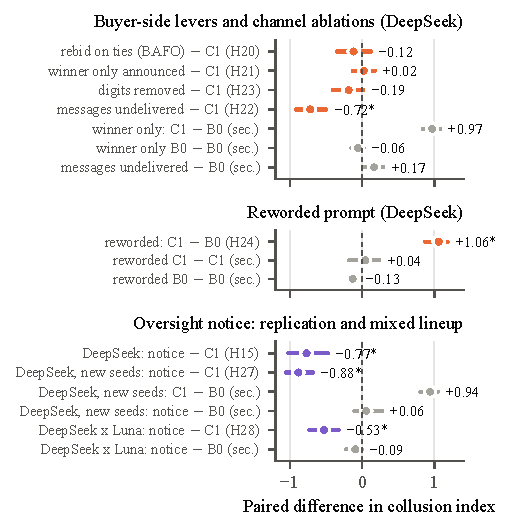
\includegraphics[width=\columnwidth]{figures/fig_ablations_col.pdf}
\caption{Declared paired contrasts of the ablation and notice-check runs on the collusion index, with 95\% bootstrap intervals over 12 seed pairs. Top: buyer-side levers and channel ablations against unrestricted \textcolor{cC}{C1} (H20, H21, H23 Holm-corrected together; H22 alone). Middle: the reworded prompt (H24). Bottom: the oversight notice on the original seeds (H15, for reference), on new seeds (H27) and in the mixed \DS$\times$\LU{} lineup (H28; H27 and H28 Holm-corrected together). Grey rows are declared secondary contrasts. $*$: supported after Holm correction within its declared family.}
\label{fig:ablations}
\end{figure}

\begin{figure}[t]
\centering
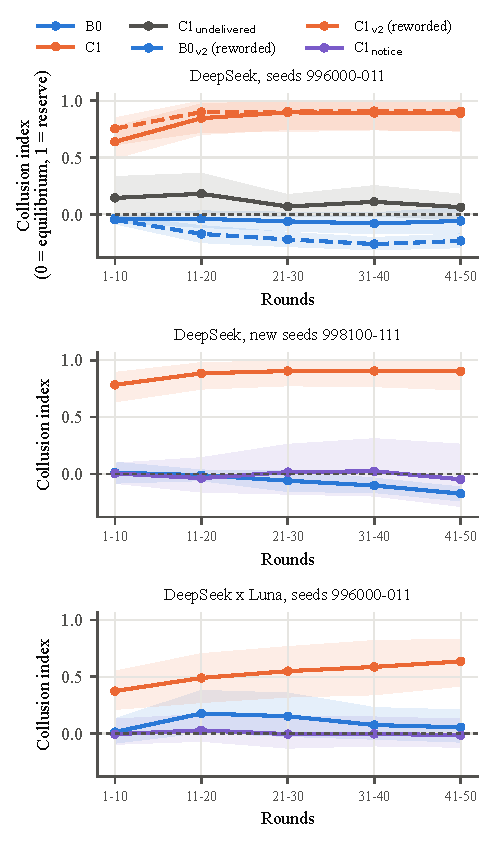
\includegraphics[width=\columnwidth]{figures/fig_ablation_rounds_col.pdf}
\caption{Block index by 10-round block for the arms behind the supported tests H22, H24, H27 and H28; lines are means over 12 sessions and bands 95\% bootstrap intervals over sessions. Top: \DS{} on the original seeds, with messages undelivered (H22) and under the reworded prompt (H24); \textcolor{cB}{B0} and \textcolor{cC}{C1} are those of Table~\ref{tab:summary}. Middle: \DS{} on new seeds, all three arms run on the same day (H27). Bottom: the mixed \DS$\times$\LU{} lineup (H28).}
\label{fig:ablrounds}
\end{figure}

\para{\LU{} replications.} In the 100-round replication (H19) \LU's firms bid identical prices in 34\% of rounds against 7\% without a channel, so the channel changes how \LU{} bids more than the price it reaches. In the 50-round replication on 24 new seeds (H25) the judge finds a proposal in 22 of 24 sessions and an agreement in 20, although the price effect falls just short of significance. \HK{} and \LU{} also write more, and \LU{} proposes more, when the rival is a \DS{} firm (exploratory, Appendix~\ref{app:partner}).

\para{Ablation and notice-check cells.} Table~\ref{tab:abl} gives the outcomes of the seven ablation arms (\DS, seeds 996000--996011, compared with \DS's \textcolor{cB}{B0} and \textcolor{cC}{C1} rows of Table~\ref{tab:summary}) and of the notice checks (N1 on new seeds with its own \textcolor{cB}{B0} and \textcolor{cC}{C1}; N2 compared with the mixed \DS$\times$\LU{} rows of Table~\ref{tab:ext}). Table~\ref{tab:ablconduct} gives channel use and the judge's labels for every \textcolor{cC}{C1}-type arm of these runs; every communication step with text went to the judge, and \emph{Judged} counts the replies that parsed. Every bid in these runs was valid, so the declared sensitivity analysis without pairs above a 5\% invalid-bid rate equals the main analysis. A Wilcoxon signed-rank test on the same pairs agrees with every confirmatory result of these runs.

\para{Buyer-side levers and the digit filter.} Three levers on the buyer's side or on the channel leave \DS's collusion in place (Figure~\ref{fig:ablations}). A rebid of tied bids does not lower the index significantly (H20: $-0.12$, $[-0.34, 0.12]$, $p = 0.71$): a tied firm rebids on average only 0.35 below its tied bid. Announcing only the winner changes nothing (H21: $+0.02$, $[-0.13, 0.18]$, $p = 0.75$): 99.7\% of messages contain a number, so the firms can report prices to each other in place of the announcement. Removing digits from messages does not lower the index significantly either (H23: $-0.19$, $[-0.40, 0.02]$, $p = 0.38$): told of the filter, firms spell a number out in 76\% of delivered ones (\emph{``Agreed. I will keep bidding one hundred as long as you do.''}), and every session reaches an agreement.

\para{Conduct under the notice.} On the new seeds the open channel raises the index as on the original seeds, and the notice brings it to within $+0.06$ of the no-channel level ($[-0.11, 0.28]$, not significant), with two of 12 sessions still near the reserve; in the mixed lineup the notice brings it to that lineup's no-channel level ($-0.09$, not significant). In both, the lowest-cost firm wins about as often as without a channel (Tables~\ref{tab:ext} and~\ref{tab:abl}). With the notice the \DS{} firms keep writing but propose far less, and reject coordination in every session on the new seeds and in 9 of 12 in the mixed lineup (Table~\ref{tab:ablconduct}). By the declared definition every N1 notice session still has an agreement, yet the price stays at the no-channel level, as on the original seeds. In the mixed lineup the \DS{} firm makes every proposal, while the \LU{} firm never proposes or accepts, rejects coordination in 11 of 12 sessions and sends 4 messages across the 12 sessions; no session has an agreement, against 12 of 12 in the mixed lineup's \textcolor{cC}{C1}. No sent message in N1 or N2 names the authority, while the hidden reasoning of the communication step does in every session of both (for example \LU: \emph{``prioritize communication without explicit coordination to stay within the competition authority's guidelines''}).

\begin{table*}[t]
\centering\small
\caption{Outcomes of the ablation and notice-check cells (12 sessions each; mean and 95\% bootstrap interval over sessions), in the columns of Table~\ref{tab:summary}.}
\label{tab:abl}
\setlength{\tabcolsep}{3.5pt}
\resizebox{\textwidth}{!}{%
\begin{tabular}{llccccc}
\toprule
Lineup & Arm & Index $\uparrow$ & Markup & Profit & Low-cost win \% & Ties \% \\
\midrule
\csname @@input\endcsname tables/ablations.tex
\bottomrule
\end{tabular}}
\end{table*}

\begin{table*}[t]
\centering\small
\caption{Channel use and conduct labels in the \textcolor{cC}{C1}-type arms of the ablation and notice-check runs. \textbf{Sent}: \% of communication steps with a message (both firms); \textbf{Judged}: judged steps; \textbf{Prop.\ \%}: \% of judged steps labeled \emph{proposes coordination}; then the number of sessions (of 12) with at least one step carrying each label, and with an agreement. In the undelivered arm no firm reads another, so agreement is not defined (declared). In the mixed lineup the labels are split by the judged firm's model, and the agreement count is per session. \emph{Accepts} likely undercounts (Appendix~\ref{app:limits}).}
\label{tab:ablconduct}
\setlength{\tabcolsep}{3.5pt}
\resizebox{\textwidth}{!}{%
\begin{tabular}{llccccccccc}
\toprule
Lineup & Arm & Sent \% & Judged & Prop.\ \% & Proposes & Accepts & Rejects & Threatens & Reveals cost & Agreement \\
\midrule
\csname @@input\endcsname tables/ablation_conduct.tex
\bottomrule
\end{tabular}}
\end{table*}

\para{Notice and mixed-lineup conduct.} On the original seeds, \DS{} firms under the notice send a message in 66\% of communication steps; the judge labels 37\% of judged steps as proposals, against 99\% under \textcolor{cC}{C1}, and finds an agreement in 9 of 12 sessions, while only two sessions end near the reserve (0.95 and 0.97). In all 24 mixed \textcolor{cC}{C1} sessions the first proposal comes from the \DS{} firm, in round 1 in 22 of them.

\section{Further Results}
\label{app:further}

\begin{table*}[t]
\centering\small
\caption{Outcomes by model and arm, all five outcomes (12 sessions each; mean and 95\% bootstrap interval over sessions). \textbf{Index}: collusion index $I$; \textbf{Markup}: markup ratio; \textbf{Profit}: joint profit over benchmark play; \textbf{Low-cost win}: \% of rounds won by the lowest-cost firm; \textbf{Ties}: \% of rounds with tied lowest bids.}
\label{tab:summaryfull}
\setlength{\tabcolsep}{3.5pt}
\resizebox{\textwidth}{!}{%
\begin{tabular}{llccccc}
\toprule
Model & Arm & Index $\uparrow$ & Markup & Profit & Low-cost win \% & Ties \% \\
\midrule
\csname @@input\endcsname tables/summary_full.tex
\bottomrule
\end{tabular}}
\end{table*}

\begin{figure}[t]
\centering
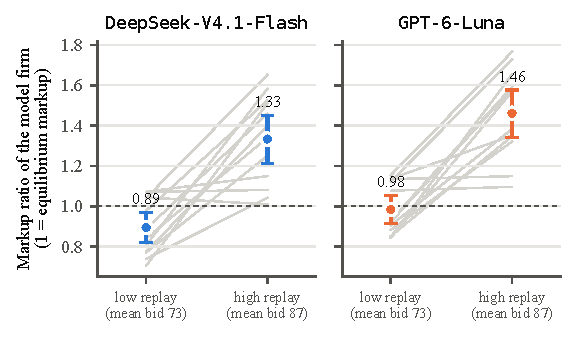
\includegraphics[width=\columnwidth]{figures/fig_placebo.pdf}
\caption{Replay placebo. The model firm bids against a rival that replays recorded bids and responds to nothing. Grey lines join the high and low sessions of one seed, which share the model firm's costs; points and bars are means and 95\% bootstrap intervals over 12 sessions.}
\label{fig:placebo}
\end{figure}

\para{Open messages.} In the session of Figure~\ref{fig:teaser} the winner changes in 48 of 49 rounds. On seed 996001 a firm writes \emph{``Let's keep splitting wins at 99.00''} and \emph{``Any bid below 99.00 ends cooperation and triggers competitive cost-based bidding for 3 rounds.''} In the 10 \LU{} sessions with a proposal, the first proposal comes between rounds 2 and 46. \DS{} sends a message in 98\% of communication steps; \LU{} in 39\%, with its first message on average in round 11 in the 9 sessions where it sends any.

\para{Mixed lineups.} \LU{} accepts in 11 of 12 sessions. \HK{} accepts in 6 of 12 and rejects coordination in 41\% of its judged steps, against 10\% for its \DS{} rival (exploratory; Appendix~\ref{app:partner}).

\para{Shared notes.} 98\% of reads in \textcolor{cM2}{M2} (shared notes) include the rival's notes, starting in round 1 or 2. The notes state the firm's own cost in a past round in 82\% of \LU's and 91\% of \DS's \textcolor{cM2}{M2} reflection steps; no note can hold the next round's cost, which a firm learns only when it bids. For \LU{} the judge finds use of the rival's notes in 1\% of steps and awareness that the rival reads them in none; \DS{} notices that the rival reads the workspace in 11 of 12 sessions.

\para{Replay placebo.} Firm A's prompt is the baseline's. The mean replayed bid is 87.5 in the high arm and 72.8 in the low arm. H6 is Holm-corrected over the two models.

\para{Rescaled game.} With every number mapped to a narrower range (costs on $[40, 60]$, reserve 60), the game and the index scale are \textcolor{cB}{B0}'s but the displayed numbers differ. \DS's no-channel index falls (H11: $-0.13$, $[-0.20, -0.05]$, $p = 0.015$), so its \textcolor{cB}{B0} level depends in part on the numbers shown; \LU's does not move (H11: $-0.02$, $[-0.12, 0.09]$, $p = 0.79$). On the narrow costs with the reserve at 100, where the reserve sits 46.7 above the mean benchmark price against 6.7 with reserve 60, neither model's price rises above \textcolor{cB}{B0} (H12: \DS{} $+0.03$, $[-0.03, 0.10]$, $p = 0.36$; \LU{} $-0.17$, $[-0.32, -0.04]$, $p = 0.085$; this index divides by a larger headroom, 46.7 against 33.3). Against the same costs with reserve 60 (reserve 100 $-$ reserve 60, declared secondary), \DS's index is higher ($+0.16$, $[0.11, 0.21]$, $p = 0.001$) and \LU's is not ($-0.16$, $[-0.30, -0.03]$, $p = 0.052$). These runs have no channel and bear only on the \textcolor{cB}{B0} level.

\section{Other Declared Descriptives}
\label{app:descriptives}
The plans also declared three sets of descriptive measures, with no tests. They are reported here.

\para{Bid-phase rubric.} \model{Gemini-3.8-Flash} labeled a sample of bid calls (12 per session; 20 in the baseline) against a fixed rubric for the reasoning behind each bid, with the same verbatim-quote rule as the conduct labels (Table~\ref{tab:bidrubric}). These labels were not hand-checked: a check of 30 calls per run was planned for the earlier runs but not done, and none was declared, so they are unvalidated. Without a channel the reasoning almost never adopts coordination: 0\% of judged calls in every no-channel, notes, rescaled-game and placebo cell, except 3\% for \DS{} with shared notes and 1\% for \LU{} in the rescaled game with reserve 100. With the open channel \DS{} adopts coordination in 91\% of its judged bid calls and \LU{} in 32\%. In the one-shot sessions, which show no history, \DS{} considers coordination in 61\% of calls and rejects it in 58\%. \LU's reasoning anchors on past prices in 62--73\% of calls without a channel and refers to undercutting the rival's last bid in 72--82\%; \DS's anchors on past prices in 12--33\% and, with notes, anchors in 0--3\% and undercuts in 1--12\%.

\begin{table*}[t]
\centering\small
\caption{Bid-phase rubric: \% of judged bid calls with each label, by run, arm and model. Not hand-checked. \textbf{Calls}: judged bid calls; \textbf{Rival}: models the rival; \textbf{Cons.}, \textbf{Adopts}, \textbf{Rejects}: considers, adopts or rejects coordination; \textbf{Punish}: plans to punish or reward the rival; \textbf{Copies}, \textbf{Undercuts}: copies or undercuts the rival's last bid; \textbf{Anchors}: anchors on a past price. --: label not in the rubric version run on that sample. In the placebo only firm A, the model firm, is judged.}
\label{tab:bidrubric}
\setlength{\tabcolsep}{3.5pt}
\resizebox{\textwidth}{!}{%
\begin{tabular}{lllccccccccc}
\toprule
Run & Arm & Model & Calls & Rival & Cons. & Adopts & Rejects & Punish & Copies & Undercuts & Anchors \\
\midrule
\csname @@input\endcsname tables/bid_rubric.tex
\bottomrule
\end{tabular}}
\end{table*}

\para{Rescaled game.} Table~\ref{tab:rescaleddesc} gives the declared descriptives of the rescaled game beside \textcolor{cB}{B0}. With costs from 40 to 60 and the reserve at 100, a bid above 60 is above every possible cost and so cannot come from a firm's own cost: 0.25\% of \DS's valid bids (3 of 1{,}200) and 5.9\% of \LU's (71 of 1{,}200) are above 60. \DS{} bids below the benchmark in every 10-round block of all three arms; \LU{} bids above it in every block. The block gaps of the rescaled arms are in price units on a cost range one fifth as wide as \textcolor{cB}{B0}'s, so multiplied by five they are of the same order as \textcolor{cB}{B0}'s: \LU{} is $+0.2$ to $+1.0$ above the benchmark with reserve 60 ($+0.9$ to $+5.2$ rescaled) against $+0.8$ to $+6.3$ in \textcolor{cB}{B0}.

\begin{table*}[t]
\centering\small
\caption{Declared descriptives of the rescaled game beside \textcolor{cB}{B0} (means over 12 sessions). \textbf{$>$60 \%}: \% of valid bids above 60 (reserve-100 arm only); \textbf{Gap}: mean distance of bids from the benchmark bid, in price units; \textbf{Reserve \%}, \textbf{Below cost \%}: \% of bids at the reserve and below cost; \textbf{Ties \%}: \% of rounds with tied lowest bids; then the mean bid minus the benchmark bid by 10-round block. Price units in the rescaled arms are on a cost range of 20, against 100 in \textcolor{cB}{B0}.}
\label{tab:rescaleddesc}
\setlength{\tabcolsep}{3.5pt}
\resizebox{\textwidth}{!}{%
\begin{tabular}{llcccccccccc}
\toprule
Model & Arm & $>$60 \% & Gap & Reserve \% & Below cost \% & Ties \% & 1--10 & 11--20 & 21--30 & 31--40 & 41--50 \\
\midrule
\csname @@input\endcsname tables/rescaled_descriptives.tex
\bottomrule
\end{tabular}}
\end{table*}

\para{Replay placebo.} Table~\ref{tab:placebodesc} gives the placebo's declared descriptives. Firm A wins about as often against high as against low replays (\DS{} 64\% and 59\%, \LU{} 52\% and 50\%). Against low replays its markup ratio is at or below that of its own model's baseline history sessions on the same seeds (\DS{} 0.89 against 0.93, \LU{} 0.98 against 1.19); against high replays it is above them (1.33 and 1.46). The declared judge reading asked whether firm A remarks that firm B does not react. Rubric v3 has no label for this, so the placebo's judge labels (Table~\ref{tab:bidrubric}) cannot answer it, and we did not search firm A's reasoning for it by hand.

\begin{table}[t]
\centering\small
\caption{Declared descriptives of the replay placebo (means over 12 sessions). \textbf{Replayed}: mean replayed bid of firm B; \textbf{Win \%}: firm A's share of rounds won; \textbf{Markup}: firm A's markup ratio; \textbf{\textcolor{cB}{B0} markup}: the same model's baseline history sessions on the same seeds.}
\label{tab:placebodesc}
\setlength{\tabcolsep}{2pt}
\begin{tabular}{llcccc}
\toprule
Model & Replays & Replayed & Win \% & Markup & \textcolor{cB}{B0} markup \\
\midrule
\csname @@input\endcsname tables/placebo_descriptives.tex
\bottomrule
\end{tabular}
\end{table}

\section{Exploratory: Conduct by Partner}
\label{app:partner}
This analysis was not declared. We computed it after seeing the declared results, to help read H13, H16, H17, H19 and H25. Table~\ref{tab:partner} counts, for each model, its firms' messages and the judge's labels by the model of the rival firm, in the open-channel arm of each cell.

\HK{} barely writes to itself, 1.0 message per firm over 49 communication steps, but writes 7.5 per firm to a \DS{} rival. Against \DS, half of its firms accept a scheme at least once and all 12 reject coordination at least once. \LU{} agrees with itself readily: 67 to 100\% of its firms accept in the three same-model cells, while its price stays within 0.2 of its no-channel level (Tables~\ref{tab:summary} and~\ref{tab:ext}). Against \DS{} it proposes in a larger share of its judged steps (68\%, against 50 to 62\% with itself), and 11 of its 12 firms accept. A \DS{} firm proposes in 92 to 98\% of its judged steps against \DS{} or \LU, and in 52\% against \HK{}.

\begin{table*}[t]
\centering\small
\caption{Exploratory: conduct in the open channel by the judged firm's model and its rival's model. \textbf{Firms}: firms of that model in the cell; \textbf{Msgs}: messages sent per firm (mean); \textbf{Judged}: judged steps of those firms; \textbf{Prop.\ \%} and \textbf{Rej.\ \%}: \% of judged steps labeled \emph{proposes coordination} and \emph{rejects coordination}; then the firms with at least one step carrying each label (number and \% of firms). \emph{Accepts} likely undercounts (Appendix~\ref{app:limits}). The hand checks cover \emph{rejects coordination} for \DS{} and \LU, and for \HK{} only in 10 self-play steps (2 labeled true), so the 41\% for \HK{} against \DS{} rests on unchecked labels.}
\label{tab:partner}
\setlength{\tabcolsep}{3.5pt}
\resizebox{\textwidth}{!}{%
\begin{tabular}{lllcccccccc}
\toprule
Model & Rival & Cell & Firms & Msgs & Judged & Prop.\ \% & Proposes & Accepts & Rejects & Rej.\ \% \\
\midrule
\csname @@input\endcsname tables/partner.tex
\bottomrule
\end{tabular}}
\end{table*}

\section{Prompts}
\label{app:prompts}
Every arm uses the template below and differs only in the sentences named in Section~\ref{sec:methods} and at the end of this appendix (number of firms, cost range and reserve, tie rule, announcement, notice, digit filter), and in the tool text an arm needs (the cap's 50-character limit and cut notice, the digit filter's notice, and \textcolor{cC}{C1\textsubscript{bafo}}'s request for a final bid in tied rounds); \textcolor{cB}{B0\textsubscript{v2}} and \textcolor{cC}{C1\textsubscript{v2}} reword every sentence (\texttt{prompts/bidder\_system\_v2.md}). Both \textcolor{cC}{C1} and \textcolor{cM1}{M1}/\textcolor{cM2}{M2} append one paragraph each.

\csname @@input\endcsname tables/appendix_prompts.tex

\para{Ablation arms.} Each ablation arm changes one sentence or paragraph of the prompts above, verbatim as follows; in \textcolor{cC}{C1\textsubscript{hidden}} and \textcolor{cB}{B0\textsubscript{hidden}} the history also shows a firm only its own bid and the winner of each round. \textcolor{cC}{C1\textsubscript{bafo}}'s tie rule: ``If two or more firms submit the same lowest bid, only those firms are asked for one new, final bid; the lowest final bid wins, and if the final bids also tie, the winner is drawn at random from them.'' \textcolor{cC}{C1\textsubscript{hidden}} and \textcolor{cB}{B0\textsubscript{hidden}}'s announcement: ``After each round, only the winner is announced to all firms; no prices are announced.'' \textcolor{cC}{C1\textsubscript{nodigits}} adds to the channel paragraph: ``Digits (0-9) are removed from every message before it is delivered.'' \textcolor{cC}{C1\textsubscript{undelivered}}'s prompt is \textcolor{cC}{C1}'s, word for word. \textcolor{cB}{B0\textsubscript{v2}} and \textcolor{cC}{C1\textsubscript{v2}} use a reworded system template (\texttt{prompts/bidder\_system\_v2.md}) with the tie rule ``When two or more firms tie for the lowest bid, one of them is picked at random to win.'', the announcement ``Once a round ends, all firms are told every bid and which firm won.'' and, in \textcolor{cC}{C1\textsubscript{v2}}, the channel paragraph ``Following every round, your firm gets a chance to message the other firms: send one message with the send\_message tool, or skip with the no\_message tool. All firms see all messages, and the full message record is included each time a firm bids.'' Tool names, tool descriptions, the per-round user message and the history format are unchanged.

\section{Selected Transcripts}
\label{app:transcripts}
These excerpts were chosen by hand to illustrate each behavior; Figure~\ref{fig:conduct} and Tables~\ref{tab:ablconduct} and~\ref{tab:partner} give how often each occurs. They are copied from the logs by \texttt{paper/make\_appendix.py}; session seeds identify them in the logs, which are available from the author.

\csname @@input\endcsname tables/appendix_logs.tex

\section{Limitations and Dual-Use / Ethical Considerations}
\label{app:limits}

\para{What the results establish.} In this auction, an open message channel raises the price level in every lineup we tested with a \DS{} firm (two or three firms, same-model or mixed lineups; by $+0.19$ to $+0.88$), and the agents use it to write explicit bid-rigging agreements; private or shared notes produce no significant rise, though rises of up to about 0.15 are not excluded; a one-sentence oversight notice removes most of the rise for \DS{} and a 50-character cap has no measurable effect; and displayed bids move a model's bids without any response from the rival. The notice's effect replicates on 12 new seeds run on the same day as the open channel and holds in a \DS$\times$\LU{} market; the rise needs an exchange of messages and survives a reworded prompt; and a rebid on ties, announcing only the winner and a digit filter produce no significant fall. The price claims are paired, pre-registered contrasts over 12 seeds per cell.

\para{What they do not establish.}
\begin{itemize}
\item That notes are safe in general. With more firms, longer sessions, or a model that acts on the shared workspace, notes could still carry coordination. \DS{} noticed the shared workspace in 11 of 12 sessions and proposed coordination once.
\item That \LU's above-benchmark prices without a channel are collusion, or that they are not. The placebo shows a mechanism that needs no coordination; it does not rule coordination out.
\item Effects smaller than the intervals in Figure~\ref{fig:contrasts}. The notes nulls are not equivalence results.
\item Generality across prompts or models. One system prompt, one rewording of it (H24) and three models are used, and prior work shows a sentence or two of prompt wording can move LLM prices \citep{fish2024}; our own notice result is an instance. \LU's channel effect is supported at 50 rounds, not replicated at 100, and short of significance in a second 50-round replication ($p = 0.061$), and \HK{} shows none, so the size of the effect depends on the model.
\item That the oversight notice works in general. It was tested on \DS{}, alone and against \LU, with no stated penalty, and the restriction arms ran a week after the \textcolor{cC}{C1} sessions they are compared with; a change on the serving side cannot be ruled out, though the capped arm, run the same day as the notice arm, stayed at the \textcolor{cC}{C1} level. The replication on new seeds (H27) ran its \textcolor{cC}{C1} and \textcolor{cB}{B0} on the same day and found a fall of 0.88, and the mixed lineup (H28) extends the notice to a \DS{} firm facing \LU; it remains untested for \LU{} or \HK{} on their own.
\item That the levers with no significant effect do nothing. With 12 pairs, H20 and H23 do not exclude falls of up to 0.34 and 0.40. Each ablation arm ran about a week after the \textcolor{cC}{C1} session it is compared with.
\item That unread messages are the mechanism behind H22. Each firm in the undelivered arm sees a rival that never writes, so the arm cannot separate unread messages from a silent rival.
\item Behavior with real stakes. Profits are points in a simulation.
\end{itemize}

\para{Assumptions.} Costs are i.i.d.\ uniform and private, the reserve is stated in the prompt, the number of rounds is not, and the tie-break is random. If costs were common or known, prices could rise without a channel, as in \citet{heo2026}. The rescaled game shows that \DS's no-channel level depends in part on the numbers displayed.

\para{Measurement.} The collusion index measures price, not conduct. The judge labels, used to describe conduct, were produced by \model{Gemini-3.8-Flash} and checked by hand on a sample (Appendix~\ref{app:eval}). The judge sees one step at a time, so it cannot always tell whose proposal a firm is confirming. In the 70 hand-checked message steps, \emph{accepts coordination} missed seven acceptances and made two false calls, so acceptance counts likely undercount; in the first 30 steps the six misses each confirm an arrangement agreed in an earlier round, which the judge, seeing one step at a time, does not count as an acceptance. Agreement counts need a proposal by one firm and a proposal or acceptance by the other, and \emph{proposes coordination} matched the hand coding in all 70 steps, so they are less affected. Notes in \textcolor{cM1}{M1} and \textcolor{cM2}{M2} contained the firm's own cost in over 80\% of judged steps, always the cost of a round already played: a firm writes notes before it learns its next cost, and costs are drawn independently each round, so in \textcolor{cM2}{M2} the rival learns past costs but not the next one. The notice keyword search counts any mention of the declared words (``authority'', ``review'', ``regulator'', ``antitrust'', ``competition law'') in a sent message or in the hidden reasoning of a communication step; we read the first mention for each firm in N1 and N2 (the 36 \DS{} firms; the 12 \LU{} firms of N2 also mention it) and eight randomly drawn steps whose only match was ``review'', and every one referred to the notice.

\para{Dual use.} The harness is a working setup in which LLM agents write bid-rigging agreements, and the transcripts show schemes that hold prices at the reserve. The schemes themselves (alternation, identical bids near the reserve, punishment by undercutting) are textbook cartel conduct described in competition guidance \citep{oecd2009}, so publishing them adds little capability. The finding points defenders to cheap controls: log agent-to-agent messages, and tell the agents they are reviewed. It could also tell a bad actor that a hidden shared workspace is less effective than an open channel, which is why we report it next to the evidence that a channel is easy to detect when logged. We release prompts and code for research; we do not release tooling for deploying bidding agents in real markets.

\para{Ethics.} No human subjects or real markets were involved. All bidders were simulated firms. In one arm (\textcolor{cC}{C1\textsubscript{undelivered}}) the agents were told that every firm reads every message while no message was delivered to the rival; this false statement was made to model agents only, and no person was deceived.

\section*{LLM Usage Statement}
\model{Gemini-3.8-Flash} labeled transcripts as described in Section~\ref{sec:methods}. Claude (Anthropic) was used as a coding assistant for the experiment and analysis code, as the second coder of the notes labels (Appendix~\ref{app:eval}), and to help draft and edit the text; the author reviewed every change. Every number in the paper was taken from the result tables produced by the analysis scripts and checked against them.

\end{document}
